\documentclass[10pt,nocopyrightspace]{sigplanconf}

% TODO: 10pt, 11pt or nothing (default: 9pt)

\usepackage{amsmath}
\usepackage[T1]{fontenc}
\usepackage{hyperref}
\usepackage{graphicx}

\begin{document}

\special{papersize=8.5in,11in}
\setlength{\pdfpageheight}{\paperheight}
\setlength{\pdfpagewidth}{\paperwidth}

\titlebanner{banner above paper title}        % These are ignored unless
\preprintfooter{short description of paper}   % 'preprint' option specified.

\title{Hailstorm: Distributed Stream Processing with Exactly Once Semantics}
\subtitle{CS240h Final Project, Spring 2014}

\authorinfo{Thomas Dimson \and Milind Ganjoo}
           {Stanford University}
           {tdimson@cs.stanford.edu \and mganjoo@cs.stanford.edu}

\maketitle

\begin{abstract}

In recent years, \textit{stream processing} has emerged as data analysis
technique to handle real-time applications where the latency of Hadoop is
inappropriate. Many popular systems, such as Twitter's Storm, provide a rigid
platform for performing distributed computations over the network. Storm-like
systems typically provide at-least-once processing with state management left
to the implementor. We present a novel distributed stream processing framework,
\textit{Hailstorm}\footnote{\url{https://github.com/hailstorm-hs/hailstorm}},
which provides a platform to perform distributed computation on streams of data
in Haskell. By restricting the class of computation to commutative monoids, our
system is able to provide exactly-once semantics with little performance loss
or added complexity.

\end{abstract}

\section{Introduction}
\label{sec:introduction}

As the Internet has evolved so have user expectations in regards to latency.
In one example, Twitter's trending topics feature allows users to see breaking
stories within minutes of their emergence. In another, Google Analytics,
administrators are able to see detailed demographic information of surfers in
real time.  The volume and velocity of the data in these systems presents
challenges to typical single-machine programs: data does not fit into memory,
and latency requirements imply that error recovery has to be automatic and
nearly instantaneous.

Like MapReduce~\cite{mapreduce} and batch processing, frameworks such as
Twitter's Storm~\cite{storm} and LinkedIn's Samza~\cite{samza} have been
created to ease the development of stream processing applications. In these
systems, events of interest are pushed into distributed queues from user-facing
applications (e.g., Twitter's web site).  As the events are popped off the
queues, the stream processing framework takes over and transforms the event
using a sequence of computations. For example, we might receive Tweets from the
queue, split on whitespace and perform a windowed count to determine topics
that are currently trending. Similar to MapReduce, developers using these
systems write algorithms that operate on individual stream \textit{units} and
emit zero or more \textit{messages} to be handled by the next stage in
computation. The frameworks distribute the events to clusters running the
computation, abstracting away the unreliable nature of the network.

This paper introduces Hailstorm, a stream processing framework in Haskell.
Unlike Storm and Samza, Hailstorm mandates that all streaming computations must
be both commutative and monoidic. Like Samza, it requires that all events must
be initially stored as messages in Apache Kafka~\cite{kafka}.  These
restrictions allow Hailstorm to make stronger processing guarantees about
events: namely, that the each event will be processed \textit{exactly} once in
the system. Furthermore, unlike Storm and Samza, state recovery under error
conditions is built-in to the framework. We utilize Haskell's purity to
guarantee that side-effects of computation are isolated to a single
\textit{sink} processor at the end of the computation sequence.


\section{Related Work}
Hailstorm's technical design is based on that of Apache Storm~\cite{storm}. 
Storm is a widely used stream processing framework for
the Java Virtual Machine (JVM) allowing developers to upload jobs for continuous
processing on a Storm cluster. Developers create a directed acyclic graph of
interconnected processing layers called a \textit{topology}.
Messages are passed between layers as
\textit{tuples}. Tuples originate in a \textit{spout}, which typically reads
off of a distributed queue and are passed between layers of \textit{bolts} which
perform computation. Each bolt receives a tuple, performs a computation, and 
emits zero or more tuples to the next layer. Unlike Hailstorm, the bolts have
may have side effects to their computation and state management / error recovery
is left up to each developer. Accordingly, the system is only able to provide 
``at least once'' guarantees for processing each message in the queue. On
component failure, Storm enters a ``tuple replay'' state where it re-sends
messages from spouts in a topology. 

The theoretical underpinings of Hailstorm are inspired by a online essay, 
``Exactly Once Semantics''~\cite{jackson2014}. Jackson, a contributor to the 
Storm framework, describes Kafka log offsets as a vector clock for the system
state. This clock allows separate processors to perform synchronized snapshots
without locking or direct communication. We further describe the offset clock 
in Section~\ref{sec:clock}.

Google's MillWheel system~\cite{millwheel} also addresses the issue of exactly
once delivery of messages in a stream processing context. Like Storm,
messages flow through layers of computation to end up at a final result.
MillWheel provides exactly-once semantics by maintaining set of recently
processed tuples, discarding those that have recently appeared. Users of
MillWheel are required to manually ensure that all computations are 
idempotent, as system failure induces message re-delivery to the same processor.

\section{Hailstorm Overview}

Figure~\ref{fig:topology} shows a complete example of a Hailstorm system used
to calculate trending hashtags in real-time using the Twitter firehose. We give
a brief overview of the various components describe them in detail in the
upcoming sections.

\begin{itemize}
\item \textit{Apache Kafka} is used as the sole queuing mechanism for
  messages. Messages are consumed off of Kafka \textit{partitions} and then
  entered into Hailstorm along with their \textit{offset} within the
  partition.

\item \textit{Spouts} are responsible for getting data into Hailstorm. Along
  with a user-specified conversion function, they consume \texttt{ByteStrings} 
  from Kafka and forward them as tuples to the next layer of computation. 

\item \textit{Bolts} are the fundamental units of computation in Hailstorm.
  Bolts take a user-specified pure monoidic operation which takes a (state, input-tuple) 
  pair and produces a (state, output-tuple) pair. Bolt state is periodically 
  persisted to the snapshot store. Figure~\ref{fig:topology} shows multiple
  layers of bolts.

\item \textit{Sinks} are the final stage of Hailstorm processing. Like bolts,
  sinks take tuples from the previous layer and perform user-specified computation. 
  However, unlike bolts, the computation runs inside the IO monad allowing the
  user to connect Hailstorm to the real world: databases, web services or even the
  console. 

\item \textit{Topologies} are user-specified directed acyclic graphs which
  describe how bolts, spouts and sinks connect together.

\item \textit{Apache Zookeeper} is used as a global service registry for
  Hailstorm. Processors are registered as into Zookeeper and removed whenever
  failures occur. 

\item \textit{The negotiator} in Hailstorm manages the state of a topology: it is
  responsible for negotiating tuple snapshots and performing error recovery. The
  negotiator itself maintains no state: if it dies, it can be resumed on any
  machine with no data loss.
\end{itemize}

\subsection{Apache Kafka}

Kafka~\cite{kafka} is fantastic.

Haskakafka\footnote{\url{http://hackage.haskell.org/package/haskakafka}}
\
\subsection{Apache Zookeeper}

Zookeeper~\cite{zookeeper} is the best.

\subsection{Clock}
\label{sec:clock}

\subsection{Spouts}

\subsection{Bolts}

\subsection{Sinks}


\begin{figure}
\centering
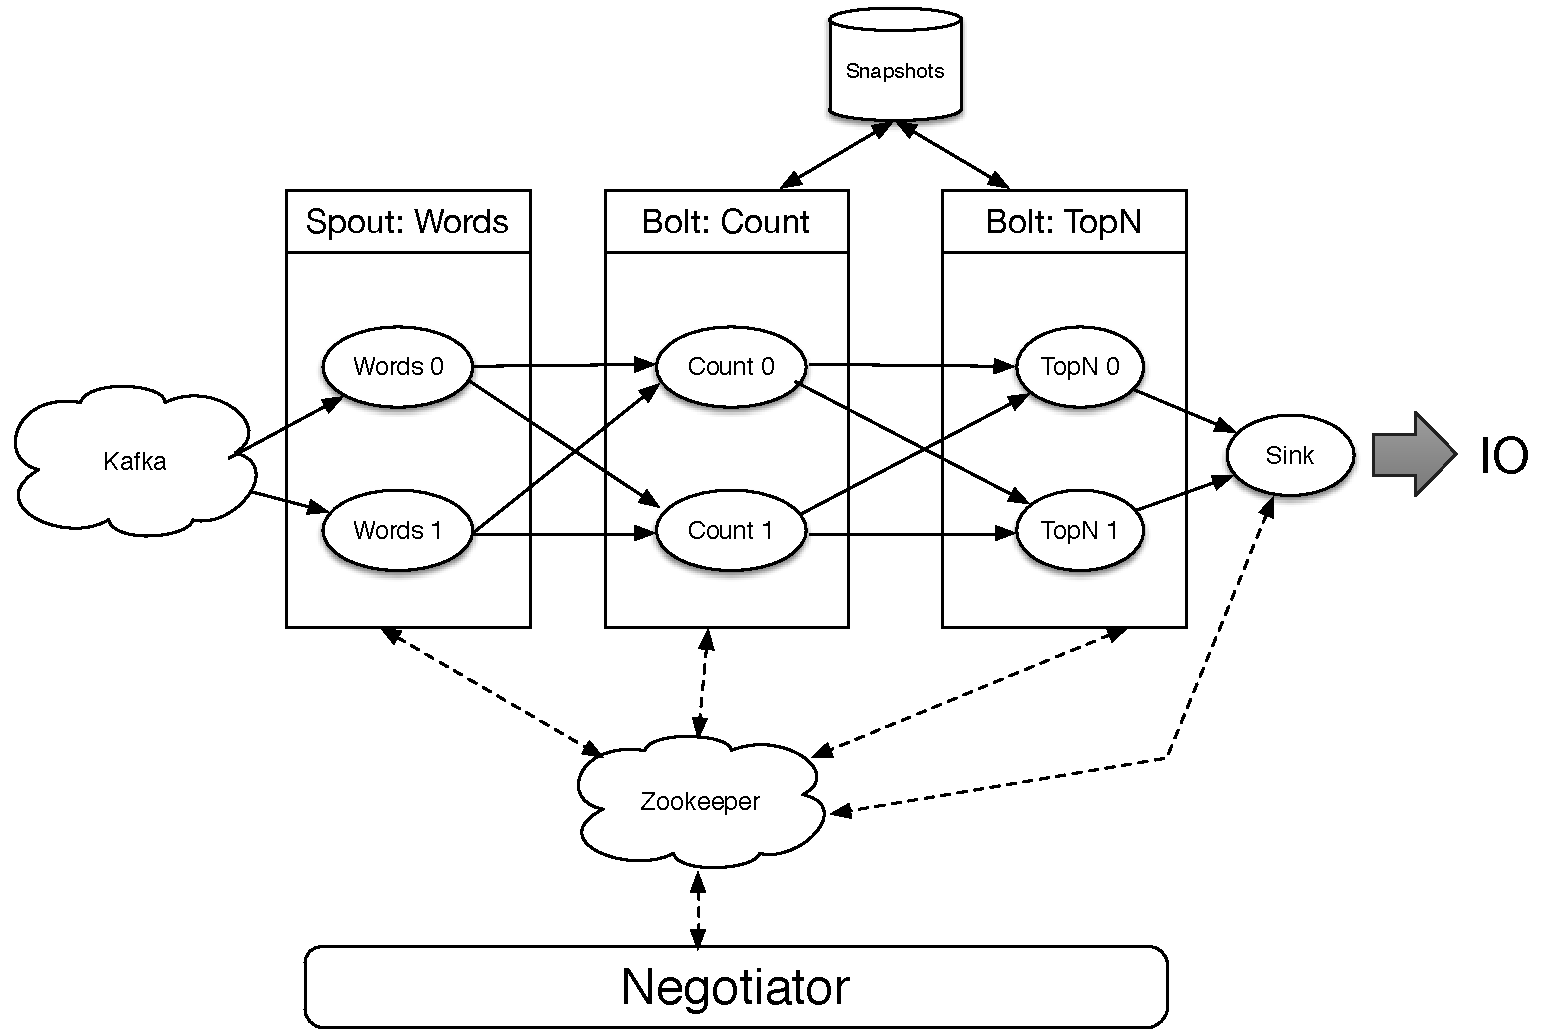
\includegraphics[width=0.5\textwidth]{images/architecture.pdf}
\caption{An example Hailstorm topology for word counts}
\label{fig:topology}
\end{figure}

\subsection{Example Topology}
Talk in detail about how hashtag counting works.

\section{Next Steps}

\section{Conclusion}

\bibliography{hailstorm}{}
\bibliographystyle{abbrvnat}

\end{document}
